\documentclass[12pt, titlepage]{article}

\usepackage{booktabs}
\usepackage{tabularx}
\usepackage{hyperref}
\usepackage{graphicx}
\hypersetup{
    colorlinks,
    citecolor=black,
    filecolor=black,
    linkcolor=black,
    urlcolor=blue
}
\usepackage[round]{natbib}

\title{SE 3XA3: Software Requirements Specification\\PROJECT TETRIS}

\author{Team \#11, Team Tetra
		\\ Daniel Agostinho agostd
		\\ Anthony Chang changa7
		\\ Divya Sridhar sridhad
}

\date{October 11, 2016}

%% Comments

\usepackage{color}

\newif\ifcomments\commentstrue

\ifcomments
\newcommand{\authornote}[3]{\textcolor{#1}{[#3 ---#2]}}
\newcommand{\todo}[1]{\textcolor{red}{[TODO: #1]}}
\else
\newcommand{\authornote}[3]{}
\newcommand{\todo}[1]{}
\fi

\newcommand{\wss}[1]{\authornote{blue}{SS}{#1}}
\newcommand{\ds}[1]{\authornote{red}{DS}{#1}}
\newcommand{\mj}[1]{\authornote{red}{MSN}{#1}}
\newcommand{\cm}[1]{\authornote{red}{CM}{#1}}
\newcommand{\mh}[1]{\authornote{red}{MH}{#1}}

% team members should be added for each team, like the following
% all comments left by the TAs or the instructor should be addressed
% by a corresponding comment from the Team

\newcommand{\tm}[1]{\authornote{magenta}{Team}{#1}}


\begin{document}

\maketitle

\pagenumbering{roman}
\tableofcontents
\listoftables
\listoffigures


\begin{table}[bp]
\caption{\bf Revision History}
\begin{tabularx}{\textwidth}{p{3cm}p{2cm}X}
\toprule {\bf Date} & {\bf Version} & {\bf Notes}\\
\midrule
October 11& 1.0 & Added Requirements\\
October 11 & 1.1 & Added Project Drivers\\
October 11 & 1.2 & Added Project Issues\\
\bottomrule
\end{tabularx}
\end{table}

\newpage

\pagenumbering{arabic}

\section{Project Drivers}

\subsection{The Purpose of the Project}
\paragraph {}
This project is to redevelop the classic game of Tetris and to ensure its compatibility with any computer. The original Tetris, created by Alexey Pajitnov in 1984, is an iconic game recognized by many gamers today. Its simplicity and minimalistic gameplay has allowed it to sell almost 500 million copies to date and is consider the best-selling paid-downloaded game of all time. 
Our product will be able to bring simple entertainment for users who are looking for games that are not too complex yet still containing a challenging element. The goal of this project will be to recreate this classic game using Java and to properly document all processes involved in its creation. The advantage of using Java would be that any computer capable of running the language will be able to play the game. This means it is not restricted to a single operating system but can be run on Windows, Mac OS, or Linux.

\subsection{The Stakeholders}

\subsubsection{The Client}
\paragraph{}
The client of our project is an external entity that is acting as both the commissioner and the reviewer since they control whether the final product is to be deployed or not. They are interested in bringing our redevelopment of Tetris for public use.
\subsubsection{The Customers}
\paragraph{}
The customer of our project is the general public. This means that anyone who is interested in video games can be considered a customer. A typical customer would be someone who has access to the internet to acquire our game and any satisfactory controller or interface to play it on. Since our product does not contain any graphical or mature content, it should be accessible to people of all ages.

\subsection{Mandated Constraints}
\subsubsection{Solution Constraints}
\paragraph{}
Description: The product shall operate on computer systems that can run Java (i.e. Windows, Mac OS, Linux)

Rationale: The client should be using the latest version of Java

Fit Criterion: Our game will be available on systems with Java and if it does not, a recommendation or link to download from the Java website will be provided

Description: The product should be playable on all computer systems without an active internet connection

Rationale: The client should be able to acquire the product either using an existing internet connection or a transfer of files from a physical drive.

Fit Criterion: The product will execute if the necessary files are stored locally on the computer. If the user has enough storage space the application will run

Description: The product can resize and adjust based on the users desired dimensions and orientation

Rationale: The client is able to resize the game window and the application will adjust accordingly unless it has hit a hard boundary

Fit Criterion: The product is to be able to change sizes on all devices regardless of the user's monitor's size and resolution. A maximum/minimum length will be predetermined in order to maintain a payable state.
\subsubsection{Partner or Collaborative Applications}
The product does not have any direct partnership or collaborative applications. The only reliance it has is to be able to be acquired through a web browser and for the existing system to support Java. A text and photography editor may be needed to create certain elements in the game.

\subsubsection{Off the shelf}
The following off-the-shelf software is required: a web browser (A preexisting one comes with any OS), Java (Available from https://java.com/en/download/), and a client for the game to run (i.e. computer with windows or Linux).

\subsubsection{Anticipated Workplace Environment}
The anticipated workplace environment for this product is any location with an accessible computer. This could potentially mean everywhere since it could reside in a permanent location, such as a person's house or office, or in a mobile environment with a laptop. The product will only be inaccessible if the client has no means of acquire the program either through the internet or physically transferring over a flash drive.

\subsubsection{Schedule Constraints}
A schedule constraint is not applicable to the development of this project. A deadline, however, has been set as a goal and the product is desired to be completed by early December.

\subsubsection{Budget Constraints}
A budget is not applicable in this case since we are given all resources to redevelop this project and it will be based on open-source code. Any additional components will have to be purchased at the cost of the developers.
\subsubsection{Enterprise Constraints}
This game will be free-to-play and does not require the user to purchase anything. The only requirement would be for the user to have access to a piece of hardware to download the game and run it (ex. A computer).


\subsection{Naming Conventions and Terminology}

\begin{table}[!h]
	\centering
	\begin{tabular}{l|l}
	Terminology & Definition\\
	CW & Clockwise \\
	CCW & Counterclockwise\\
	Tetrimino & A geometric shape composed of four squares. \\ & the classification of the seven different Tetris pieces used.\\
	Java & Object-Orientated programming language used for this project\\
	\end{tabular}
	\caption{Naming Conventions and Terminology.}
	\label{table:term}
\end{table}


\subsection{Assumptions}

\subsubsection{Business Rules}
A business rule that we have created and agreed upon is that all members of the group should have equal amount of work and participation but should take initiative if they feel they are stronger or have expertise in certain/relevant areas.

\subsubsection{Assumptions}
A few assumptions for the project is that a suitable text and photography editing software will be accessible for them to use in addition to an integrated development environment for the code to be written in. 

\section{Functional Requirements}

\subsection{The Scope of the Work and the Product}
People search for a means to escape reality and enjoy themselves while engaged in a challenge. PROJECT TETRIS will allow for those people to do just that. This is a project that will consist of designing a game in Java based on the original Tetris game. This project will be completed by December 7, 2016.
\subsubsection{The Context of the Work}
\begin{figure}
	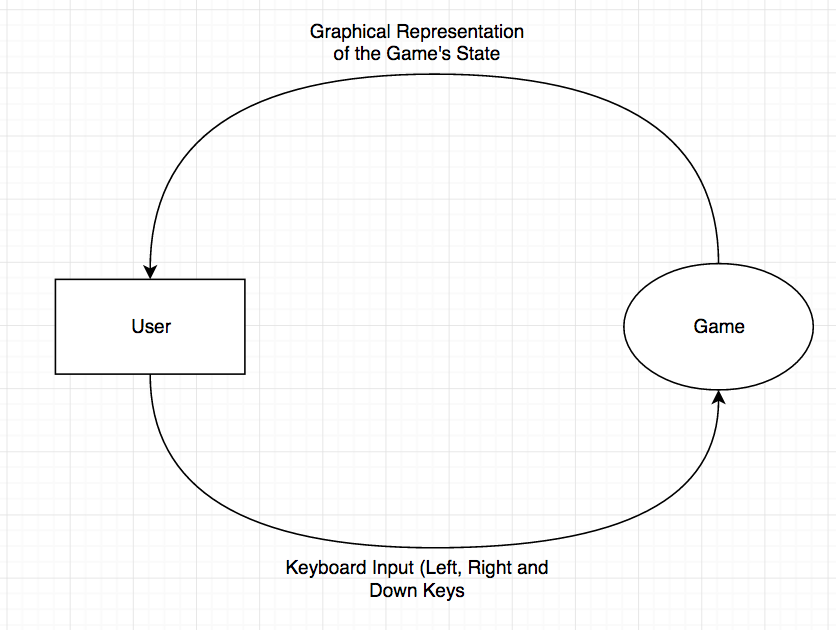
\includegraphics[width=\linewidth]{fig1.png}
	\caption{Context diagram.}
	\label{fig:context}
\end{figure}
Figure \ref{fig:context} shows the Context Diagram for this project. 


\subsubsection{Individual Product Use Cases}

\paragraph{Title: Player Moves Left}
\paragraph{}
Trigger: User presses the left key
\paragraph{}
Pre-condition: Game is in play and there is available space to the left (ie the Tetrimino is already not at the left border).
\paragraph{}
Post-condition: The Tetrimino is shifted one space to the left.

\paragraph{Title: Player Moves Right}
\paragraph{}
Trigger: User presses the right key

Pre-condition: Game is in play and there is available space to the right (ie the Tetrimino is already not at the right border).
\paragraph{}
Post-condition: The Tetrimino is shifted one space to the right.

\paragraph{Title: Player Rotates Tetrimino CW}
\paragraph{}
Trigger: User presses the Up key
\paragraph{}
Pre-condition: Game is in play and there is available space around the Tetrimino in all directions.
\paragraph{}
Post-condition: The Tetrimino is rotated 90 degrees clockwise.

\paragraph{Title: Player Rotates Tetrimino CCW}
\paragraph{}
Trigger: User presses the Down key
\paragraph{}
Pre-condition: Game is in play and there is available space around the Tetrimino in all directions.
\paragraph{}
Post-condition: The Tetrimino is rotated 90 degrees counter-clockwise.

\paragraph{Title: Player Completes a Row}
\paragraph{}
Trigger: User moves a Tetrimino into place where one or more squares from the Tetrimino complete a row of squares.
\paragraph{}
Pre-condition: Game is in play and there are existing squares in the row.
\paragraph{}
Post-condition: That row is cleared from the game and the resulting arrangement of squares on the screen shift one row 
downwards.

\paragraph{Title: Player Loses Game}
\paragraph{}
Trigger: A Tetrimino is placed with a square that is above the vertical limit.
\paragraph{}
Pre-condition: Game is in play.
\paragraph{}
Post-condition: The game is ended and the player loses.

\subsection{Functional Requirements}

\paragraph{Requirement 1: FR1}
The user must be able to move the falling Tetrimino to the left and right.
\subparagraph{Rationale:}
In order to strategically place the Tetrimino where the user desires, the Tetrimino must be able to be moved by the user.
\paragraph{Requirement 2: FR2}
The user must be able to accelerate the falling Tetrimino downwards.
\subparagraph{Rationale:}
Once the user has decided where they want the Tetrimino, they should not have to wait for the full duration of the Tetrimino falling. Also, accelerating the Tetrimino adds to the score making the accelerating feature a strategy for the user to get more points.
\paragraph{Requirement 3: FR3}
The user must not be able to move the Tetrimino in an upwards direction.
\subparagraph{Rationale:}
The challenge of the game is to strategically place the blocks under the constraint that the time and space is limited because the block is falling slowly towards the bottom of the screen.
\paragraph{Requirement 4: FR4}
The game allows the user to rotate the Tetrimino 90 degrees.
\subparagraph{Rationale:}
This allows the user to maneuver the Tetrimino into positions that they desire while still maintaining the square shape of the resulting structure.
\paragraph{Requirement 5: FR5}
The game will eliminate a row of the Tetrimino pieces if they span the entirety of the row. The resulting pieces will shift down one row to fill the vacancy.
\subparagraph{Rationale:}
The purpose of the game is place the Tetriminos such that when an entire row of squares is filled, that row is removed. Else the screen would just fill up without any resolution.
\paragraph{Requirement 6: FR6}
The Tetriminos cannot go past the border of the screen.
\subparagraph{Rationale:}
Mentioned earlier, the objective is to place the Tetriminos under a constraint of space and time. If there are no bounds or the Tetriminos can go past the boundaries, then the game has no purpose.
\paragraph{Requirement 7: FR7}
The game will end when any square should reach the row of origin.
\subparagraph{Rationale:}
The objective of the game is to get as many points before the Tetriminos reach the top of the screen. If any square from the Tetrimino should reach above a certain height. The game will be over.

\section{Non-functional Requirements}
\subsection{Look and Feel Requirements}
\paragraph{Requirement 8: NFR1}
The game must look and feel like the original Tetris game. 
\subparagraph{Rationale:}
Since PROJECT TETRIS is based off of the original Tetris game, in turn PROJECT TETRIS must look and feel like the original Tetris game. Tetris has been around for a long time and is very popular. It is recognized widely therefore playing PROJECT TETRIS should be intuitive.

\subsection{Usability and Humanity Requirements}
\paragraph{Requirement 9: NFR2}
The game should be easy to understand and able to be played without reading instructions.
\subparagraph{Rationale:}
Since PROJECT TETRIS is based off of the original Tetris game, it should be just as easy to play. To users playing PROJECT TETRIS should be intuitive. The game should have simple mechanics to be understood by all stakeholders.

\subsection{Performance Requirements}
\paragraph{Requirement 10: NFR3}
The game should be easy to understand and able to be played without reading instructions.
\subparagraph{Rationale:}
Since PROJECT TETRIS is based off of the original Tetris game, it should be just as easy to play. To users playing PROJECT TETRIS should be intuitive. The game should have simple mechanics to be understood by all stakeholders.

\subsection{Operational and Environmental Requirements}
\paragraph{Requirement 11: NFR4}
The game must be run on a computer that is running Java.
\subparagraph{Rationale:}
The game was designed in Java and therefore needs to be compiled with a Java compiler. It will not be able to run otherwise.

\subsection{Maintainability and Support Requirements}
\paragraph{Requirement 12: NFR5}
The game should support Windows, OS X and Linux.
\subparagraph{Rationale:}
Our stakeholders are not limited to running the game on only one platform. Our stakeholders can have any type of computer and still be able to run the game.

\subsection{Security Requirements}
There are no security requirements associated with PROJECT TETRIS.

\subsection{Cultural Requirements}
\paragraph{Requirement 13: NFR6}
PROJECT TETRIS will not include any images or messages that will offend parties of any culture or religion.
\subparagraph{Rationale:}
PROJECT TETRIS is intended for every type of person regardless of age or background. The user should not be subject to seeing offensive images or messages.

\subsection{Legal Requirements}
\paragraph{Requirement 14: NFR7}
PROJECT TETRIS is not an original works nor will it be distributed for sale.
\subparagraph{Rationale:}
PROJECT TETRIS is based on an open source version of Tetris. It does not mean to infringe on any copyrights. It does not claim to be original.

\subsection{Health and Safety Requirements}
\paragraph{Requirement 14: NFR7}
PROJECT TETRIS should be used under the correct physical conditions and safely.\subparagraph{Rationale:}
Since this is a game primarily for the computer, it is important to keep in mind proper ergonomics while utilizing the computer for any purpose. This includes things like proper posture, choosing the right environment, and so on.


\section{Project Issues}

\subsection{Open Issues}
At this stage of the development of our application, a lot remains unresolved. As far as the game itself goes, we need to ensure that we adhere to the rules and regulations of Tetris itself, as it is a very widely popular game recognized around the world. Furthermore, our investigation into what platform this application is focused on must also be completed; it would be best to create it as a java application that runs across all operating systems, but further research must be done on the required libraries for our project.
\subsection{Off-the-Shelf Solutions}
Currently, there exist several versions of Tetris that are widely available to play, both on the web or offline as applications to install on one's computer. This game also exists as multiple different mobile applications for various platforms, and many such versions of this game are open-source and readily available to build off of. We will use these as reference.
\subsection{New Problems}
There are none at the moment.
\subsection{Tasks}
Our task first and foremost is to set up a Model-View-Controller architecture, such that each aspect of this game can be worked on in a modular fashion. For the proof-of-concept demonstration, we want to be able to implement a basic graphical view of our game, showing at least the game board itself and depicting the various Tetrimino pieces. We also want there to be basic functionality in terms of movement of various pieces and any response to keyboard or mouse input.
\subsection{Migration to the New Product}
This is not applicable in the scope of this project.
\subsection{Risks}
There are several risks with creating and running our application, both to do with developing and testing our application. In order to be functional, our application must have no compile errors and run smoothly without crashing, or without interfering with any other applications. Furthermore, the project team must understand how to best create automated tests for this application. 
\subsection{Costs}
There are no costs involved at the moment.
\subsection{User Documentation and Training}
User documentation for this application will be available and is crucial to the user, in the form of help menus and instructions on how to play Tetris. It may also be wise to implement a short tutorial at the start of the user's gameplay experience, such that one who is new to Tetris is able to easily understand and play the game. 


\bibliographystyle{plainnat}

\bibliography{SRS}

\newpage

\section{Appendix}

The format that we used for this document was a modified version of the SRS template included in the class repo. We removed unnecessary sections.

%\subsection{Symbolic Parameters}

%The definition of the requirements will likely call for SYMBOLIC\_CONSTANTS.
%Their values are defined in this section for easy maintenance.


\end{document}